\noindent{}This work was created with \XeLaTeX. The main text is set in
the Google Droid fonts. All typewriter text is typeset in DejaVu Mono.
1.click dash home, search for "language support"
2.click "install/remove language" and add Chinese
3.click dash home, search for "keyboard input method"
4.under "input method",add Chinese input method  

\section{Software used in creating this book}
\noindent{}Pictorial materials are created using \index{graphic tools} like \index{graphic tools!Gimp}{Gimp}, \index{graphic tools!Gimp}{Gimp} and \index{graphic tools!InkScape}{InkScape}. Publishing sofware is and \index{CJK}{CJK},\index{中文LaTex}{中文LaTex}. The prgamming languages used in this are \index{Go}{Go},\index{Bash}{Bash},\index{Python}{Python}. 

\begin{itemize}
\item{GNU make \qquad\url{http://www.gnu.org/software/make/}}
GNU Make is used to automate the dependency and sequence of  different tools when making this \LaTeX  book.
\item{Dia  \qquad\url{http://dia-installer.de}} \index{Dia}{Dia} is used to create the network digram used in this book.
\item{Gimp \qquad\url{http://www.mikespook.com/learning-go/>}}
\item{InkScape \qquad\url{http://www.mikespook.com/learning-go/>}}
\item{xelatex  \qquad\url{http://www.mikespook.com/learning-go/>}}
\item{Go  \qquad\url{http://www.mikespook.com/learning-go/>}}
\item{Bash  \qquad\url{http://www.mikespook.com/learning-go/>}}
\item{Python  \qquad\url{http://www.mikespook.com/learning-go/>}}
\item{Perl  \qquad\url{http://www.mikespook.com/learning-go/>}}

\end{itemize}

\section{Install \TeX Live Environment in Ubuntu 12.04}

\begin{lstlisting}[language=Bash]
for i in \
dia graphiz gimp inkscape gnumeric \
ttf-droid ttf-dejavu ttf-sazanami-gothic \
ttf-arphic-ukai  texlive-full \
latex-cjk-xcjk git-core make \
;do 
sudo apt-get install $i -y; 
done
\end{lstlisting}

\section{Install \TeX Live Environment in Lbuntu 14.04}
texlive-2013 is used in Lbuntu-14.04.

\begin{Verbatim} [frame=lines,framesep=5mm,label={[Start of code] End of code}]
for i in \
dia graphiz gimp \
inkscape  gnumeric \
ttf-droid ttf-dejavu ttf-sazanami-gothic ttf-arphic-ukai \
texlive-lang-cjk \
texlive-fonts-recommended texlive-extra-utils texlive-xetex 
texlive-latex-extra texlive-latex-recommended \
texlive-metapost-doc texlive-metapost latex-cjk-all  git-core make lmodern pgf
do 
sudo apt-get install -y $i  
done

\end{Verbatim}

\begin{lstlisting}[language=Bash]
\end{lstlisting}

\section{Ubuntu: find Perl package}
% basicstyle is to set the font size 
\lstset{basicstyle=\tiny\color{blue}}
\begin{lstlisting}[language=Bash]
tjyang@640m:~\$ apt-cache search perl XML::Simple
libxml-simple-perl - Perl module for reading and writing XML
libdns-zoneparse-perl - Perl extension for parsing and manipulating DNS Zone Files
libgtk2-gladexml-simple-perl - clean object-oriented perl interface to Gtk2::GladeXML
libtemplate-plugin-xml-perl - XML plugins for the Template Toolkit
libtest-xml-simple-perl - Perl testing framework for XML data
libxml-libxml-simple-perl - Perl module that uses the XML::LibXML parser for XML structures
libxml-simpleobject-enhanced-perl - Perl module which enhances libxml-simpleobject-perl
libxml-simpleobject-perl - Objectoriented Perl interface to a parsed XML::Parser tree
ruby-xml-simple - Simple Ruby API for reading and writing XML
tjyang@640m:~\$ 
\end{lstlisting}


\section{Book creation flowchart}
The following people have helped to make this book what it is today.

\begin{figure}[H]
\caption{Book creation flow chart}
\label{bookmaking.dia}
\begin{center}
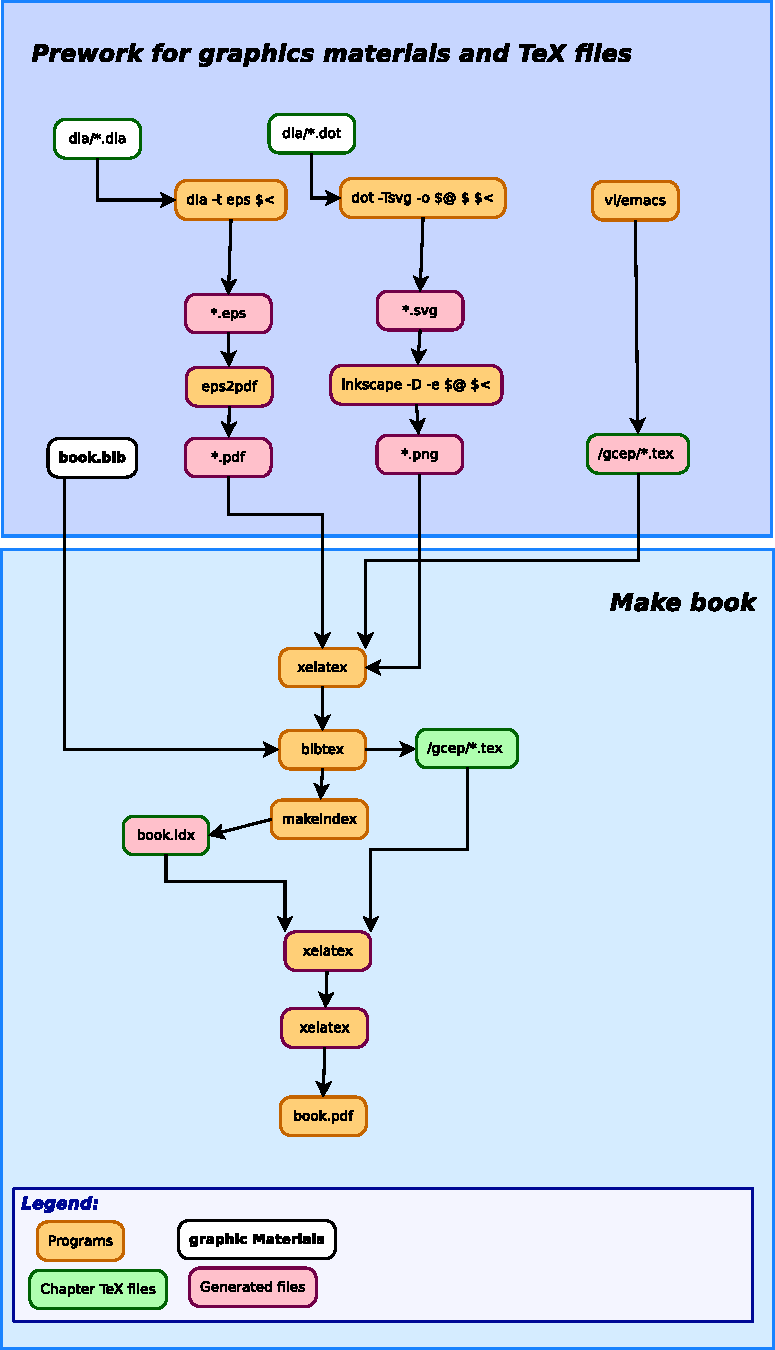
\includegraphics[scale=0.9]{dia/bookmaking.pdf}
\end{center}
\end{figure}

\section{Checking out book source}
This book is hosted on github.com. Following is the procedure to check out and request a pull request for merging  modification from you local git repository.
\begin{itemize}
\item{Get github account if not already done so}.
\item{Initiate a fork from github.com/tjyang/bananapi}.
% basicstyle is to set the font size 
\lstset{basicstyle=\tiny\color{blue}}
\begin{lstlisting}[language=Bash]
tjyang@640m:~$ cat .netrc
machine code.google.com login gname@gmail.com password XXXXXXX
tjyang@640m:~$ 
\end{lstlisting}

\item{check out your forked bananapi src}.
\begin{Verbatim} [frame=lines,framesep=5mm,label={[Start of code] End of code}]
tjyang@640m:~$ git clone git@github.com:tjyang/bananapi.git 
tjyang@640m:~$ 
\end{Verbatim}

\item{Commit your local changes and push to your github }.
\item{Send out a pull request}.

\end{itemize}


\section{Contributors}
The following people have helped to make this book what it is today.
\begin{itemize}
\item{T.J. Yang \qquad\url{<tjyang2001@gmail.com>}}.
\end{itemize}

Help with proof reading, checking exercises and text improvements (no
particular order and either real name or an alias):
\emph{T.J. Yang}


The following people provided smaller improvements, like nits, typos and
other tweaks:
%% smaller stuff, like nits, typos and other stuff
\emph{Daniele Pala}.


\subsection{T.J. Yang}
%\begin{wrapfigure}{r}{0.3\textwidth}
%  \begin{center}
%  \includegraphics[width=3cm]{fig/avatar-author-300x300}
%  \end{center}
%\end{wrapfigure}

T.J. Yang is interested about small computer like \index{RPi}RPi and \index{BPi}BPi.



\section{License and copyright}
This work is licensed under the Attribution-NonCommercial-ShareAlike 3.0 Unported License. To
view a copy of this license, visit \url{http://creativecommons.org/licenses/by-nc-sa/3.0/}
or send a letter to Creative Commons, 171 Second Street, Suite 300, San
Francisco, California, 94105, USA.\newline
All example code used in this book is hereby put in the public domain.

\copyright T.J. Yang 2012.
